%
% File: chap01.tex
% Author: Victor F. Brena-Medina
% Description: Introduction chapter where the biology goes.
%
\let\textcircled=\pgftextcircled
\chapter{Apktool}
\label{chap:apktool}

\initial{A} tool for reverse engineering 3rd party, closed, binary Android apps. It can decode resources to nearly original form and rebuild them after making some modifications. It also makes working with an app easier because of the project like file structure and automation of some repetitive tasks like building apk, etc.

It is NOT intended for piracy and other non-legal uses. It could be used for localizing, adding some features or support for custom platforms, analyzing applications and much more.

%=======
\section{Application}
\label{sec:sec0201}

\subsection{Features}
\begin{enumerate}
\item{Disassembling resources to nearly original form (including resources.arsc, classes.dex, 9.png. and XMLs)}
\item{Rebuilding decoded resources back to binary APK/JAR}
\item{Organizing and handling APKs that depend on framework resources}
\item{Smali Debugging (Removed in 2.1.0 in favor of IdeaSmali)}
\item{Helping with repetitive tasks}
\end{enumerate}


\subsection{Requirements}

The application requires only Java 1.7 (JRE 1.7) and some basic knowledge of Android SDK, AAPT and the Smali language alongside some in depth understanding of computer architecture, assembler and hexadecimal numbers.

\subsection{Installation}

 The install process is very straight forward, 


% \label{subsec:subsec01}

% Begins a subsection.

% %A figures matrix.
% \begin{figure}[t!]
% \centering
% \begin{minipage}{3.3cm}
%     \centering
%     \subtop[]{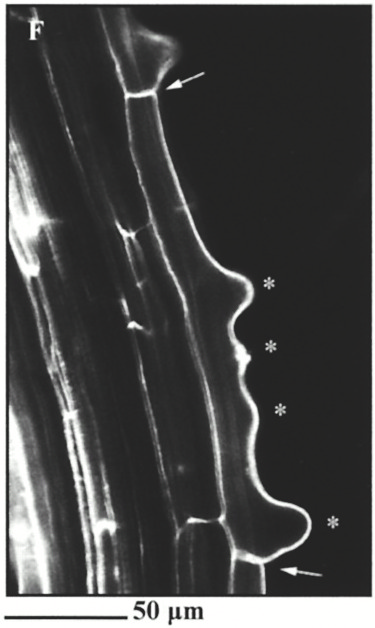
\includegraphics[height=0.28\textheight]{fig01/Nswellings}\label{sf:multiRH02a}}
% \end{minipage}
% \hspace{0.5cm}
% \begin{minipage}{3.3cm}
%     \centering
%     \subtop[]{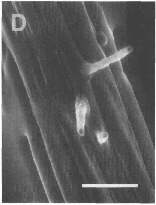
\includegraphics[height=0.27\textheight]{fig01/Mswellings}\label{sf:multiRH02b}}
% \end{minipage}
% \hspace{1.3cm}
% \begin{minipage}{3.3cm}
%     \centering
%     \subtop[]{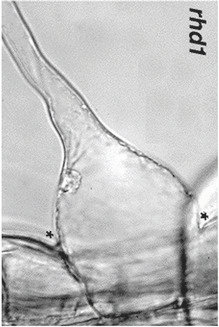
\includegraphics[height=0.27\textheight]{fig01/rhd1}\label{sf:multiRH02c}}
% \end{minipage}
% \\ \vspace{0.1cm}
% \begin{minipage}{10cm}
%     \centering
%     \subtop[]{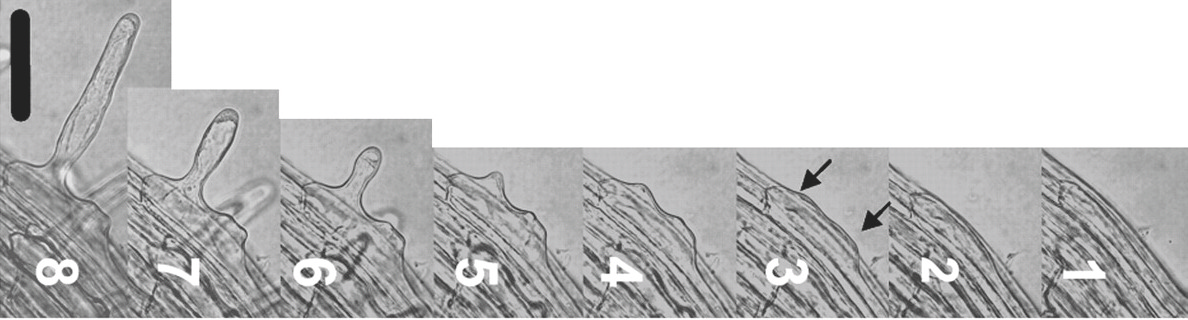
\includegraphics[height=0.145\textheight]{fig01/mutantrhd6}\label{sf:multiRH02d}}
% \end{minipage}
% \\ \vspace{0.1cm}
% \begin{minipage}{10cm}
%     \centering
%     \subtop[]{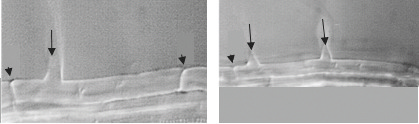
\includegraphics[height=0.16\textheight]{fig01/auxab}\label{sf:multiRH02e}}
% \end{minipage}
% \mycaption[Hair-forming mutant cells.]{(a) A mutant RH cell. Asterisks show multiple sites of RH initiation in a single root hair cell (indicated by the arrows). Figure reproduced from \cite{rigas01}. (b)~Hair-forming cell with three RH initiation locations. The bar represents $50\mu m$. Figure reproduced from \cite{massuci01}. (c) Large bump in mutant {\itshape rhd1}. Figure reproduced from \cite{griersonRH}. (d) Mutant overexpressing gene {\itshape ROP2}; from right-hand to left-hand, numbers indicate progressive snapshots at different times. RH initiation sites are indicated by the arrows. The bar represents $75\mu m$. Figure reproduced from~\cite{mjones01}. (e)~Mutants affected by auxin. On the left-hand side, RH site is farther away from the apical end (left arrow cap); on the right-hand side, multiple RH locations (arrows). Figure reproduced from~\cite{payne01}.}
% \label{fig:multiRH02}
% \end{figure}

% % A single figure
% \begin{figure}[t!]
% 	\centering
% 	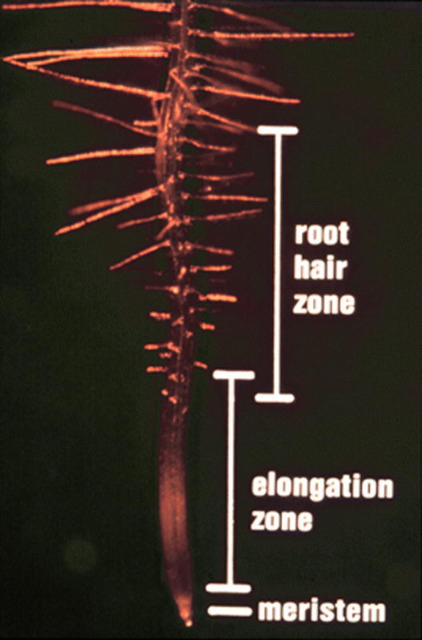
\includegraphics[height=0.35\textheight]{fig01/devepzones}
% 	\mycaption[Developmental zones of an Arabidopsis root.]{Developmental zones of an Arabidopsis root. Figure reproduced from \cite{griersonRH}.}
% 	\label{fig:RHP02}
% \end{figure}

%=========================================================